\chapter{Deep Learning, Anomaly Detection, and Hierarchical Temporal Memory}
\label{sec:background}
The following is relevant background information on Deep Learning, Video Anomaly Detection, and HTM theory.
\section{Deep Learning}
As mentioned in the introduction, deep learning has seen increased popularity in the past few years. Surprisingly enough, the field of deep learning can be traced back to 1958 when the Perceptron\cite{perceptron,perceptron2} was first introduced.
\subsection{Perceptron}
The perceptron\cite{perceptron, perceptron2} was a machine learning algorithm that was based on a simplification of the theory, at the time, about the inner workings of a neuron. The perceptron consists of three parts; the inputs $\mathbf{x}$, the weights $\mathbf{w}$, and the unit step activation function, which is shown in \autoref{fig:perceptron}.
\begin{figure}[H]
    \centering
    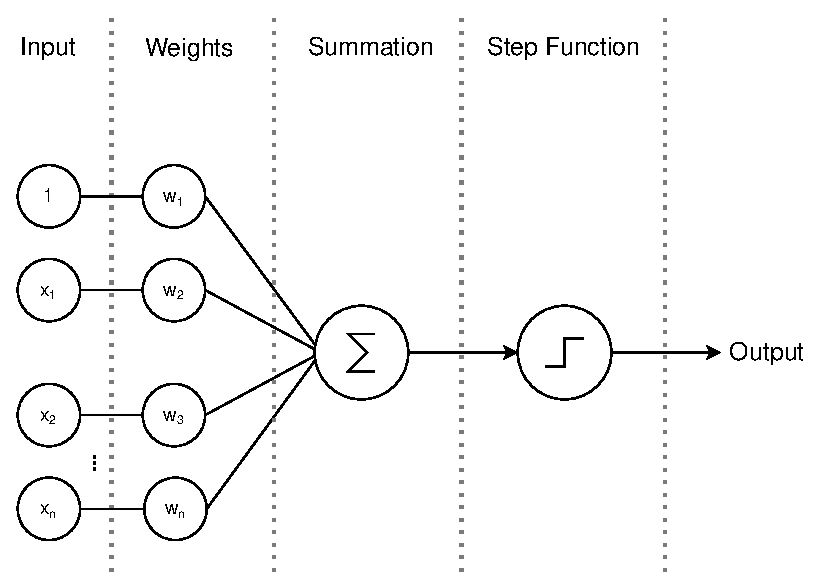
\includegraphics[width=\linewidth]{resources/related_works/perceptron}
    \caption[The Original Perceptron]{The original perceptron.}
    \label{fig:perceptron}
\end{figure}
It also requires a label $y$ corresponding to the input $\mathbf{x}$. The perceptron predicts the label of the input $\mathbf{x}$ to be $\hat{y}=sign(\mathbf{x}\cdot\mathbf{w})$. If $\hat{y}\neq y$ then it updates the weights $\mathbf{w}=\mathbf{w}+y\mathbf{x}$, otherwise it leaves $\mathbf{w}$ unchanged. This is performed until the perceptron reaches convergence, which would happen when all the inputs can be correctly classified. In other words, the perceptron requires that the inputs are linearly separable.
\par
As shown by \textcite{perceptron3}, the perceptron was able to solve linearly separable problems such as the OR function, but was unable to solve the XOR function. For the latter, it was theorized by others that stacking perceptrons in multiple layers, known as a \gls*{g_mlp}, which is shown in \autoref{fig:mlp}, would be able to solve more complex problems such as the aforementioned XOR function~\cite{perceptron_misconceptions}.
\par
\begin{figure}[H]
    \centering
    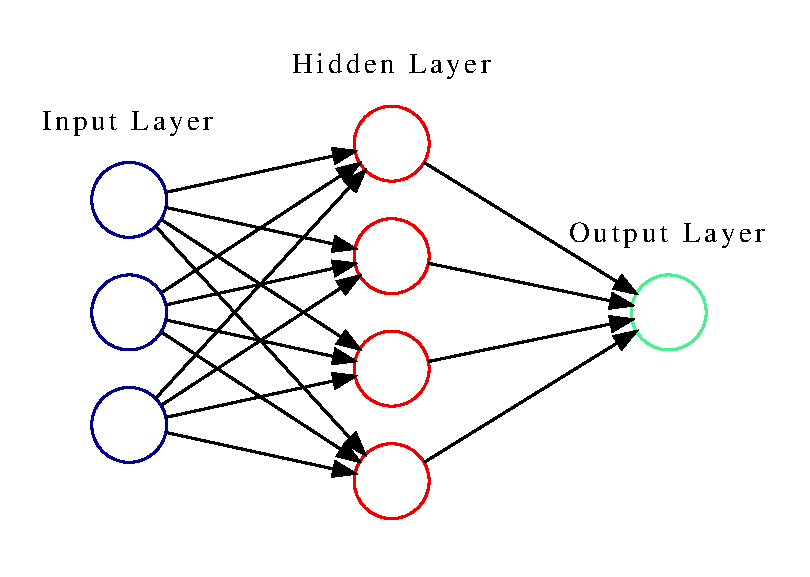
\includegraphics[width=\linewidth]{resources/related_works/mlp.gv.eps}
    \caption[MLP Example]{Example of a \gls*{g_mlp}.}
    \label{fig:mlp}
\end{figure}
Unfortunately, the work by \textcite{perceptron3} lead to the misconception that a \gls*{g_mlp} would have the same limitations as a single perceptron, and that further progress was impossible, which lead to the perceptron and other neuron-based approaches being largely abandoned~\cite{perceptron_misconceptions}. This misconception, combined with a lack of computing power and no good approaches to train a \gls*{g_mlp}, lead to a decline in the research of neuron-inspired approaches.
\par
It was not until the late 1980s~\cite{perceptron_misconceptions} that the \gls*{g_mlp} approach experienced a revival, led by the increase in computational power and the introduction of backpropagation by \textcite{backprop}, which allowed multilayer networks to be easily trained, and gave birth to modern neural networks.
\subsection{Backpropagation}
Backpropagation~\cite{backprop}, which is shorthand for "backward propagation of errors",  is a method for efficiently calculating the gradient of the error function, so that it is possible to adjust each individual weight with the purpose of lowering the error. The error function is a function that quantifies the difference between a prediction and the corresponding label, and is differentiable. An example of such an error function, is the \gls*{g_mse}:
\begin{align*}
    MSE=\frac{1}{n}\sum_{i=1}^n (y_i-\hat{y}_i)^2
\end{align*}
The result is that no longer did researchers have to manually engineer features, but could instead apply backpropagation to have the neural network automatically learn internal representations that expressed nontrivial features. An example is that no longer did researchers have to use line detection algorithms, instead the \gls*{g_mlp} could learn to represent a collection of pixels as a line automatically.
\subsection{Neural Networks}
Modern \gls*{g_mlp} networks, often referred to as just "neural networks", are similar to the \gls*{g_mlp} networks made in the 80s. The main difference is that each neuron in a \gls*{g_mlp} can have an arbitrary activation function, such as the sigmoid function and the \gls*{g_relu}~\cite{relu} function, which adds nonlinearity into the neural network and allows it to solve complex problems. They also contain more hidden layers, as seen in \autoref{fig:nn}, hence the term \emph{deep} learning.
\begin{figure}[H]
    \centering
    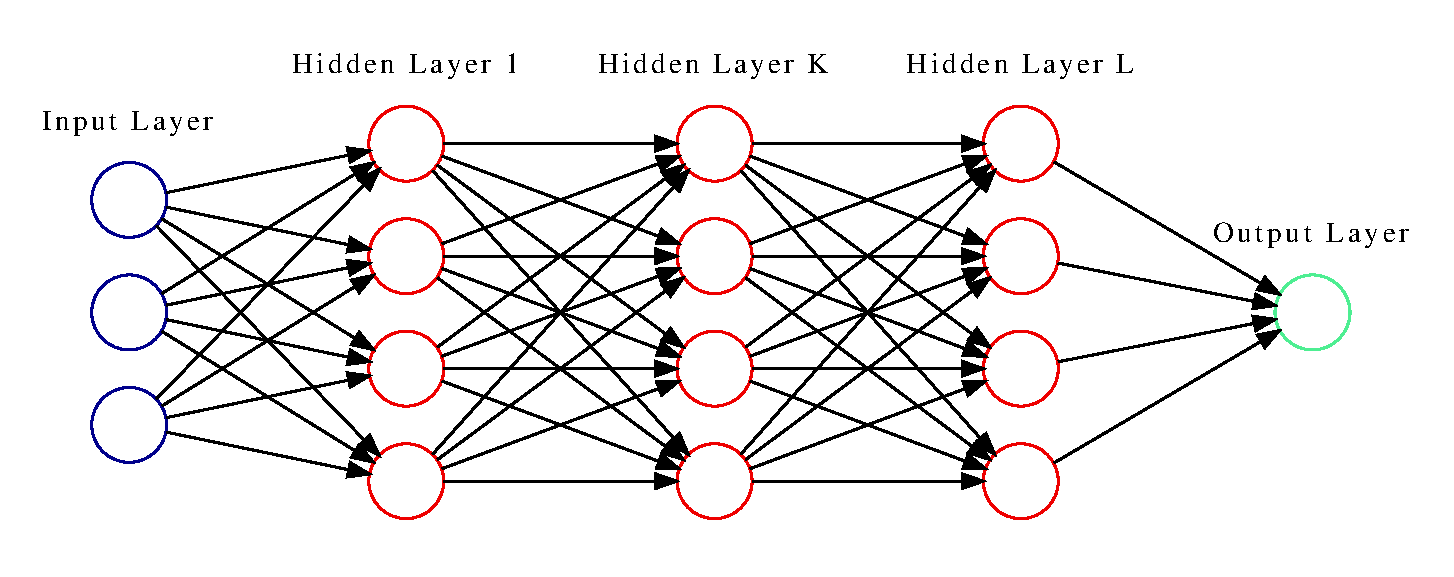
\includegraphics[width=\linewidth]{resources/related_works/nn.gv.eps}
    \caption[Neural Network Example]{Example of a neural network.}
    \label{fig:nn}
\end{figure}
\subsubsection{Learning}
Neural networks use gradients to learn. The gradients are first calculated using backpropagation which are then used to update the weights with the goal of reducing the error. This can be achieved using gradient descent, where one would calculate the gradient and descend towards the optimum using the entire dataset, but this is computationally expensive. An alternative is to use an optimizer such as \gls*{g_sgd}~\cite{sgd}, which calculates the gradient and descends using a random subset of the dataset. A visual comparison between the two methods is visualized in \autoref{fig:gd_sgd}:
\begin{figure}[H]
    \centering
    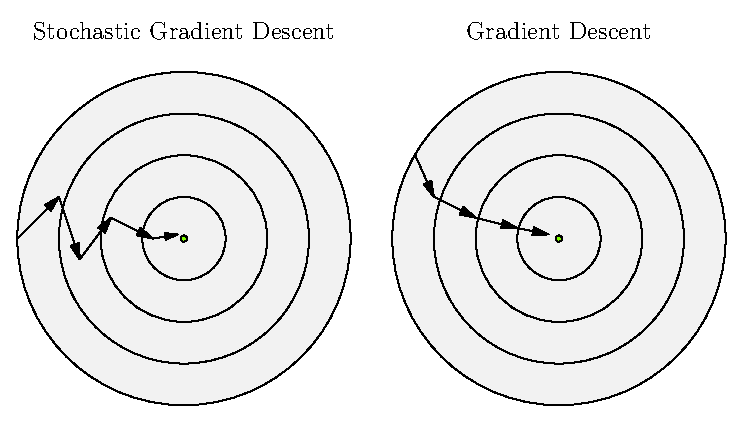
\includegraphics[width=0.8\linewidth]{resources/related_works/gradient_descent}
    \caption[Gradient Descent Comparison]{Comparison between \gls*{g_sgd} and gradient descent.}
    \label{fig:gd_sgd}
\end{figure}
\par
Yet with all the advancements within the field of neural networks, it still did not have the popularity that can be observed today. There are several reasons for this, one of them arguably being the introduction of the modern Support Vector Machine (SVM)~\cite{svm}, which overshadowed neural networks~\cite{kuncheva2019pattern}.
\par
The other reason is that neural networks did not have a lot of applications at the time, this being due to a lack of invariances which caused poor performance in machine vision, and no proper way to represent features across time which caused poor performance in time-series modelling. There was also a lack of regularization methods, which caused the models to overfit and generalize poorly. Additionally, large networks suffered from vanishing or exploding gradients~\cite{exploding_vanishing_gradients}.
\par
In order to improve upon regularization, techniques such as Dropout~\cite{dropout}, \gls*{g_bn}~\cite{batchnorm}, and Data Augmentation~\cite{data_augmentation} were introduced. New neural network architectures were invented, such as the \gls*{g_ae}~\cite{autoencoder}, that forces the model to construct an internal representation under constraints, which has a regularizing effect.
\par
As for representing features across time, architectures such as \glspl*{g_rnn}~\cite{lstm,gru} were invented. Later, attention~\cite{attention}-based models, such as the Transformer~\cite{transformer} model, were introduced.\par
The vanishing and the exploding gradient problem was alleviated by implementing, among other techniques, residual connections~\cite{resnet} between layers.
\subsection{Convolutional Neural Networks}
In an attempt to solve the problems regarding invariance and to improve the performance in machine vision tasks, \glspl*{g_cnn} were introduced by \textcite{cnn} in 1998. A \gls*{g_cnn} offers several properties that are useful, such as translational invariance~\cite{cnn}. These properties stem from the three architectural ideas in a CNN:
\begin{itemize}
    \item Local receptive fields
    \item Shared weights
    \item Spatial sub-sampling
\end{itemize}
Through the use of data augmentation, it is also possible to not only improve the effectiveness of the aforementioned invariances, but to also introduce a degree of rotational and scale invariance. A typical CNN architecture is shown in \autoref{fig:cnn_example}.
\begin{figure}[H]
    \centering
    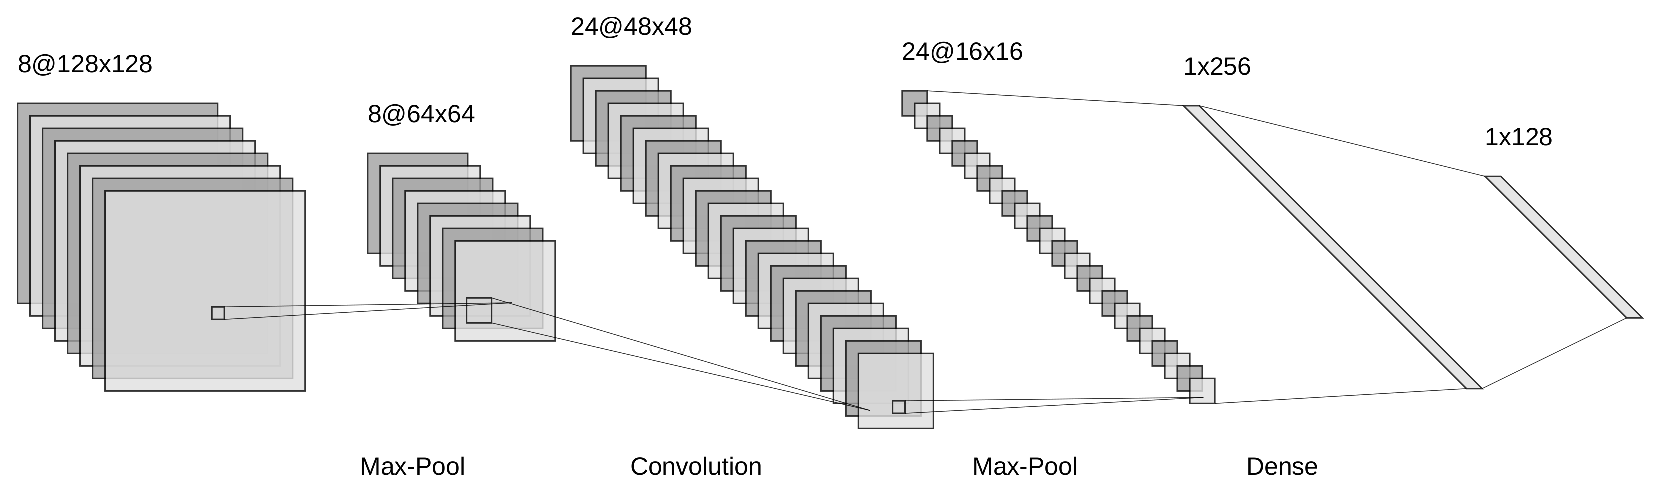
\includegraphics[width=\linewidth]{resources/related_works/cnn}
    \caption[Typical CNN Architecture]{ A typical CNN architecture. }
    \label{fig:cnn_example}
\end{figure}
\par
However, the progress within the context of machine vision stagnated due to a lack of computing power when training large models as well as a lack of sufficiently large datasets. This stagnation lasted until 2012 when AlexNet was introduced by \textcite{alexnet}, which marked a major turning point in the history of deep learning, as their record-breaking results proved that deep learning was they way forward for solving complex machine learning problems.
\par
In addition to creating a unique \gls*{g_cnn} architecture, they also made it run on a GPU and made the code publicly available. This was not the first case of running deep learning on a GPU~\cite{deeplearning_gpu}, but it can be argued that it was this paper that popularized it.  Using GPUs meant that a vast amount of computational power, for the purpose of training deep learning models, became unlocked. This also paved the way for frameworks such as PyTorch~\cite{pytorch} and Tensorflow~\cite{tensorflow}, which have democratized deep learning and made it into what it is today.
\subsection{Generative Models}
Some of the latest progress within deep learning can be attributed to generative models, such as \glspl*{g_gan}~\cite{gan} and \glspl*{g_vae}~\cite{vae}. Generative models take some input, and then generate realistic output. The input could be anything from random noise to a real sample.
\par
The idea is that generative models learn a distribution which describes the data domain represented by the training data, and can then generate synthetic data from that distribution by simply sampling it.
\par
Generative models come in all shapes and sizes, but a standard \gls*{g_gan} usually consists of just a generator and a discriminator. The generator takes some inputs (usually some random noise) and generates some samples. The batch of generated samples are then combined with a batch of real samples and mixed up. The discriminator then has to decide for every sample whether it is real or generated. This is essentially a two-player game in which the generator attempts to fool the discriminator. A typical \gls*{g_gan} pipeline is shown in \autoref{fig:gan} below.
\begin{figure}[H]
    \centering
    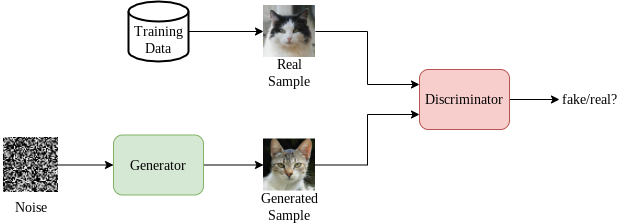
\includegraphics[width=\linewidth]{resources/related_works/gan.png}
    \caption[Gan Example]{Example of a \gls*{g_gan}.}
    \label{fig:gan}
\end{figure}
In order to train the weights in such a configuration, the generator and discriminator are trained in alteration. To train the discriminator, the weights of the generator are fixed and backpropagation is performed using the error based on whether the discriminator made the right prediction. To train the generator, the weights of the discriminator are fixed and backpropagation is performed using the error based on whether the discriminator was fooled or not.
\par
While the training method of a \gls*{g_gan} is straight forward, actually training a \gls*{g_gan} well is hard and faces several challenges such as mode-collapse, non-convergence, and instability~\cite{gan_challenges,gan_challenges2}. To alleviate these challenges, modifications to the standard \gls*{g_gan} have been proposed such as the Wasserstein GAN~\cite{wgan} and the Unrolled GAN~\cite{unrolled_gan}.
\par
There also exists variations of the standard \gls*{g_gan} for the purpose of different types of generation. One example is the CycleGAN~\cite{CycleGAN} which makes it possible to perform domain translation, such as turning a horse in an image into a zebra, without paired data. Another example is CGAN~\cite{cgan}  in which both the generator and discriminator are conditioned on some auxiliary information, which makes it possible to generate data within a specific context. For instance, instead of generating arbitrary human faces, a CGAN can generate faces of a specific age.
\subsection{Disadvantages of Deep Learning}
A disadvantage for deep-learning models in general is that they are susceptible to noise in the dataset~\cite{noise1,noise2}, which leads to decreased classification accuracy and poor prediction results.
\par
Due to the nature of training deep learning models, they are also in most cases not self-supervised and therefore require constant tuning in order to stay effective on changing data. Not to mention that they require a lot of data before they can be considered effective, and that performance increases logarithmically based on the volume of training data~\cite{deeplearning_dataset}. This is visualized in \autoref{fig:data_size_accuracy}.
\begin{figure}[H]
    \centering
    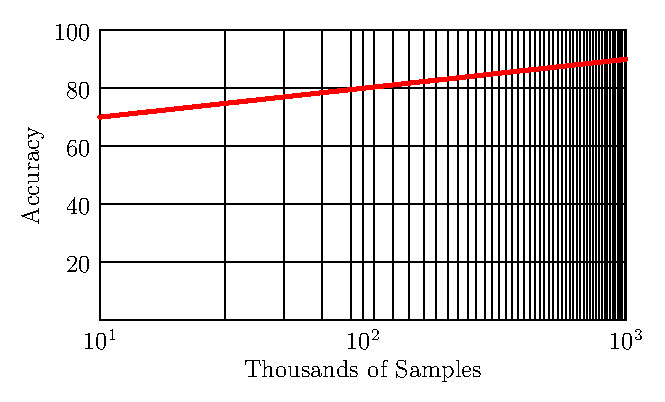
\includegraphics[width=0.8\linewidth]{resources/related_works/training_volume}
    \caption[Dataset Volume Accuracy]{Accuracy increase in relation to size of dataset.}
    \label{fig:data_size_accuracy}
\end{figure}
Deep learning models also suffer from issues with out-of-distribution performance, where a model might perform great on the dataset it is tested on, but performs poorly when deployed in real life. This could be caused by selection bias in the dataset or when there are differences in the causal structure between the training domain and the deployment domain~\cite{deeplearning_ood}.
\subsubsection{Explainability}
As stated by \textcite{XAI}, as "black-box" approaches such as deep learning surged in popularity, many realized that they offered poor explainability. While it is known \textit{how} the models make their decisions, their huge parametric spaces make it unfeasible to know \textit{why} they make those predictions. Combined with the vast potential that deep learning offers in critical sectors such as medicine, has lead to an increase in focus on developing approaches that offer explainability.
\begin{figure}[H]
    \centering
    \begin{subfigure}{0.3\linewidth}
        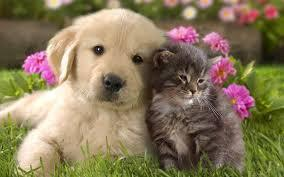
\includegraphics[width=\linewidth, height=\linewidth]{resources/related_works/gradcam_original.jpg}
    \end{subfigure}
    \hfill
    \begin{subfigure}{0.3\linewidth}
        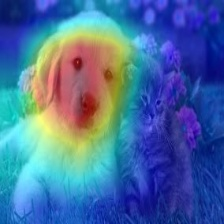
\includegraphics[width=\linewidth]{resources/related_works/gradcam_dog.jpg}
    \end{subfigure}
    \hfill
    \begin{subfigure}{0.3\linewidth}
        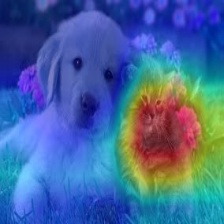
\includegraphics[width=\linewidth]{resources/related_works/gradcam_cat.jpg}
    \end{subfigure}
    \caption[Grad-Cam Visualization]{Grad-CAM visualization for the labels "dog" and "cat". Taken from~\textcite{GradCamExample}.}
    \label{fig:grad_cam}
\end{figure}
Approaches such as Grad-CAM~\cite{GradCam} (\autoref{fig:grad_cam}) and Guided Backpropagation~\cite{guided_backprop} offer improvements in that regard, but these approaches are not made with generative models in mind. In fact, there are very few explainable AI approaches for generative models~\cite{XAI}.
\section{Anomaly detection}
\label{sec:anomaly_detection}
As reviewed by \textcite{anomaly_detection}, anomaly detection is often defined as detecting data points that deviate from the general distribution of the data, this also often includes quantifying the level of deviation. Unlike other problems within machine learning and statistics, anomaly detection deals with unpredictable and rare events, therefore adding complexities to problems. Some complexities are as follows:
\begin{itemize}
    \item \textbf{Unknowns} Anomalies are associated with many unknowns which do not become known until the anomaly happens. \textcite{unknown_detection1,unknown_detection2} are works that address this.
    \item \textbf{Rarity and class imbalance} Anomalies are by definition rare instances, which means that it becomes difficult to create a balanced dataset. \textcite{class_imbalance1} review the current solutions to this problem.
    \item \textbf{Heterogeneity} Anomalies can take form in many ways, and as such one class of anomalies can be vastly different from another. Approaches such as the one introduced by \textcite{heterogeneous1} have been proposed to alleviate the problem.
\end{itemize}
These complexities make it hard to apply traditional deep learning methods for anomaly detection, because they are designed to be trained with pairs of $\{input, target\}$ in mind.
\subsection{Deep Learning and Anomaly Detection}
\label{sec:dl_anom_detection}
The current state-of-the-art algorithms for anomaly detection are numerous, but the main approach is achieved by using deep learning~\cite{anomaly_detection}. As previously mentioned, traditional deep learning approaches are hard to apply for anomaly detection. Instead, a popular approach is to use generative deep learning models such as GANs~\cite{anomaly_detection, ganomaly,anomalyvideo} to generate synthetic data and compare it to real data in order to detect anomalies. This approach is based on the assumption that the model will only be able to generate data similar to what it has been trained on, and therefore fail when an anomalous event occurs. A variation of GAN which is specifically designed for anomaly detection is GANomaly\cite{ganomaly}, shown in \autoref{fig:ganomaly}, which effectively compares image encoding latent space instead of image distributions.
\begin{figure}[H]
    \centering
    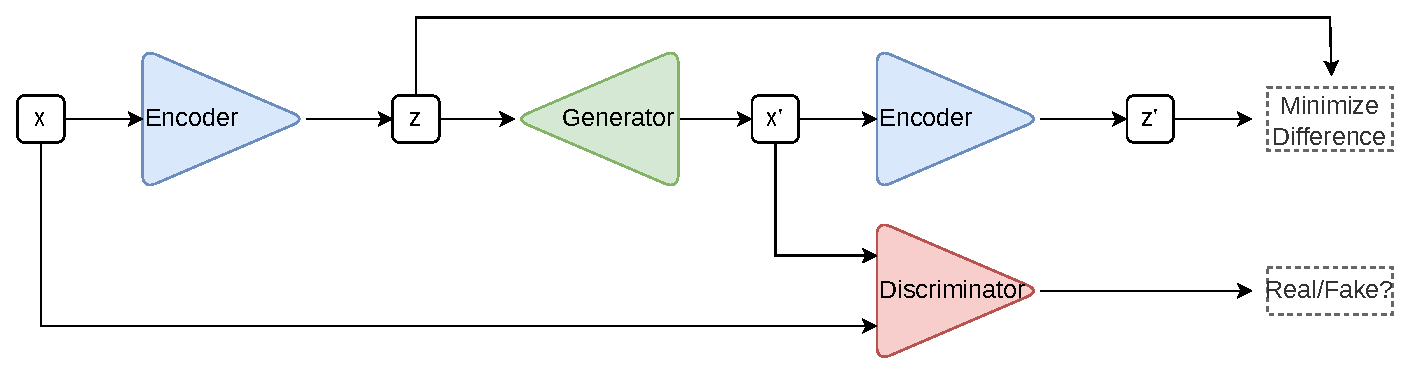
\includegraphics[width=\linewidth]{resources/related_works/ganomaly}
    \caption[GANomaly Visualization]{GANomaly~\cite{ganomaly}, a variation of \gls*{g_gan} for Anomaly detection.}
    \label{fig:ganomaly}
\end{figure}
The advantage is that GANs are generally good at generating realistic data, especially when it comes to images. The disadvantage is that GANs are very hard to train and may give suboptimal results given that they try to generate good synthetic data rather than directly detect anomalies. The training data also needs to contain all possible non-anomalous classes of events, which may not be a realistic expectation.
\par

Another common approach is autoencoders, which aim to minimize the reconstruction error from a learned feature representation space~\cite{autoencoder1,anomaly_detection,anomalyvideo}. The assumption is that anomalies are more difficult to reconstruct than normal data, hence the reconstruction error will be high and can therefore be used as a metric to detect anomalies.
\par
As previously stated, generative models suffer from a lack of explainability, and since generative models make up most of the state-of-the-art approaches in anomaly detection, it is safe to say that there is a lack of explainability in the field of anomaly detection. There are also variations of the aforementioned approaches, such as Adversarial Autoencoders, but the core idea is the same: To get an anomaly measure using some sort of generated or reconstructed data.
\subsection{Smart Surveillance}
Smart surveillance, which is the use of automatic video analysis specifically in surveillance, has seen rapid development since its inception. \textcite{anomalyvideo, smart_surveillance_2} present and summarize recent progress for anomaly detection in video for surveillance purposes, where the most promising methods are achieved by using convolutional \glspl*{g_ae} and \glspl*{g_gan}. More specifically, memory augmented autoencoders~\cite{memae} and future frame prediction GANs~\cite{future_frame_prediction} are some of the most promising approaches. In general, the results show that the deep learning approaches have a high degree of accuracy, and are consistently improving. This is not surprising given that generative models are popular in anomaly detection, as mentioned in \autoref{sec:dl_anom_detection}.
\par
The work by \textcite{anomalyvideo} also discusses problems with using deep learning approaches for anomaly detection, and further emphasizes the complexities mentioned in \autoref{sec:anomaly_detection}. One of the examples that it uses is about a bicycle on campus being wrongly classified as an anomaly, which is related to the aforementioned issue with the non-realistic requirement that the training data must contain all possible classes of non-anomalous events.

\section{Hierarchical Temporal Memory}
Today's machine learning algorithms aim to solve complex problems by simulating a substantial amount of mathematically defined neurons. These neurons are vastly simplified compared to the neurons in the brain and therefore do not have the complexity required to solve complex problems with an accuracy and level of generalizability comparable to the brain. \textcite{BAMI} introduces HTM theory which aims to outline a machine learning algorithm which works on the same principles as the brain and therefore solves some of the aforementioned issues.\par
The brain consists of layers that have been added throughout evolution. The inner layers are responsible for primal intelligence such as hunger, sex and instincts. HTM theory specifically aims to roughly simulate the neocortex, which is the outer layer of the brain tasked with advanced logic. It is important to note that HTM only attempts to \emph{estimate} the activity in the neocortex, unlike Spiking Neural Networks and others which aim to \emph{accurately simulate} the activity of the neocortex~\cite{spiking_neural_networks}.
\subsection{Structure}
\label{sec:htm_structure}
HTM aims to replicate the structure of the neocortex which is made up of cortical regions. Cortical regions consist of cortical columns, where each column is divided into layers height-wise. These cortical columns are made up of mini-columns, which in turn are made up of neurons. \autoref{fig:cortical_region} visualizes the structure of a cortical region according to HTM theory.
\begin{figure}[H]
    \centering
    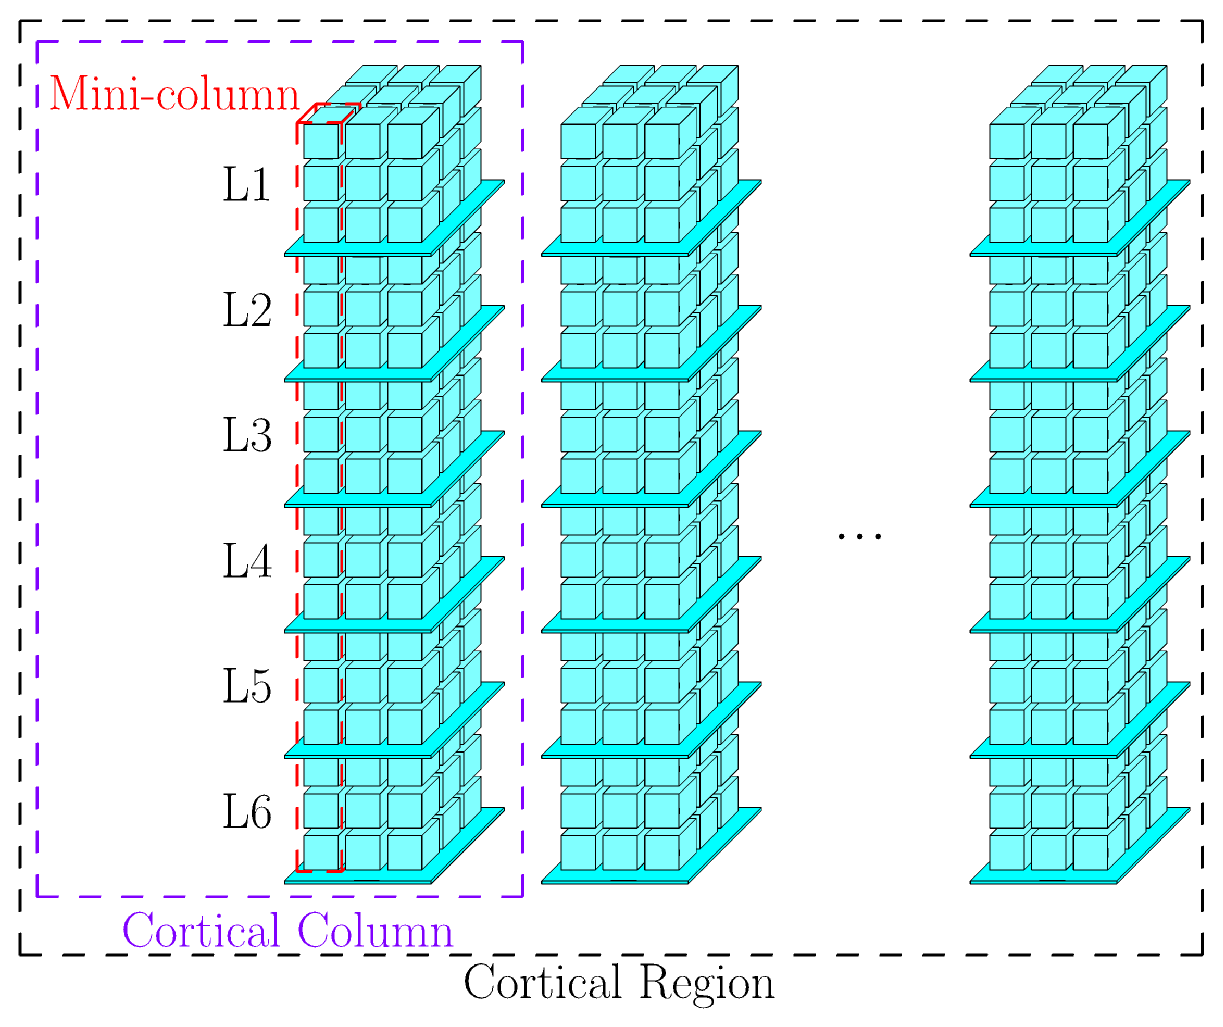
\includegraphics[width=\textwidth]{resources/related_works/cortical_region}
    \caption[HTM Structure]{Visualization of a cortical region structure in the neocortex according to HTM theory.}
    \label{fig:cortical_region}
\end{figure}
There is still uncertainty regarding the purpose, and even the existence, of each layer, but the following has been concluded~\cite{htm_l2_l3,cortical_region}:
\begin{itemize}
    \item[\textbf{L6}] Deals with input information.
    \item[\textbf{L5}] Motor outputs to body.
    \item[\textbf{L4}] Sensorimotor inference.
    \item[\textbf{L3}] Temporal Memory.
    \item[\textbf{L2}] Connects to other cortical columns and performs voting.
    \item[\textbf{L1}] Connections to cortical regions further up.
\end{itemize}
Current HTM implementations only model cortical columns, and layer-wise only L2/L3 but can be extended to model L4 as well~\cite{htm_l2_l3}.
\par
Neurons in HTM theory are different from neurons in traditional machine learning~\cite{htm_neurons}. The term neuron in traditional machine learning is very misleading and since it is mathematically derived, has actually very little in common with a biological neuron. A biological neuron does not perform back propagation but learns by strengthening and weakening inter-neural connections (synapses), which is something that the HTM neuron attempts to model through Hebbian-like learning. The difference is shown in \autoref{fig:neuron_comparison}.
\begin{figure}[H]
    \centering
    \begin{subfigure}[b]{0.35\linewidth}
        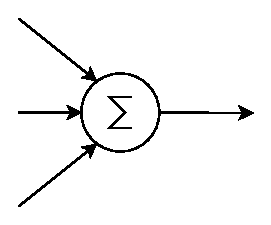
\includegraphics[width=\linewidth]{resources/related_works/neuron_ml}
        \caption{Deep learning neuron}
    \end{subfigure}\\
    \begin{subfigure}[b]{0.35\linewidth}
        \centering
        \hspace*{1cm}
        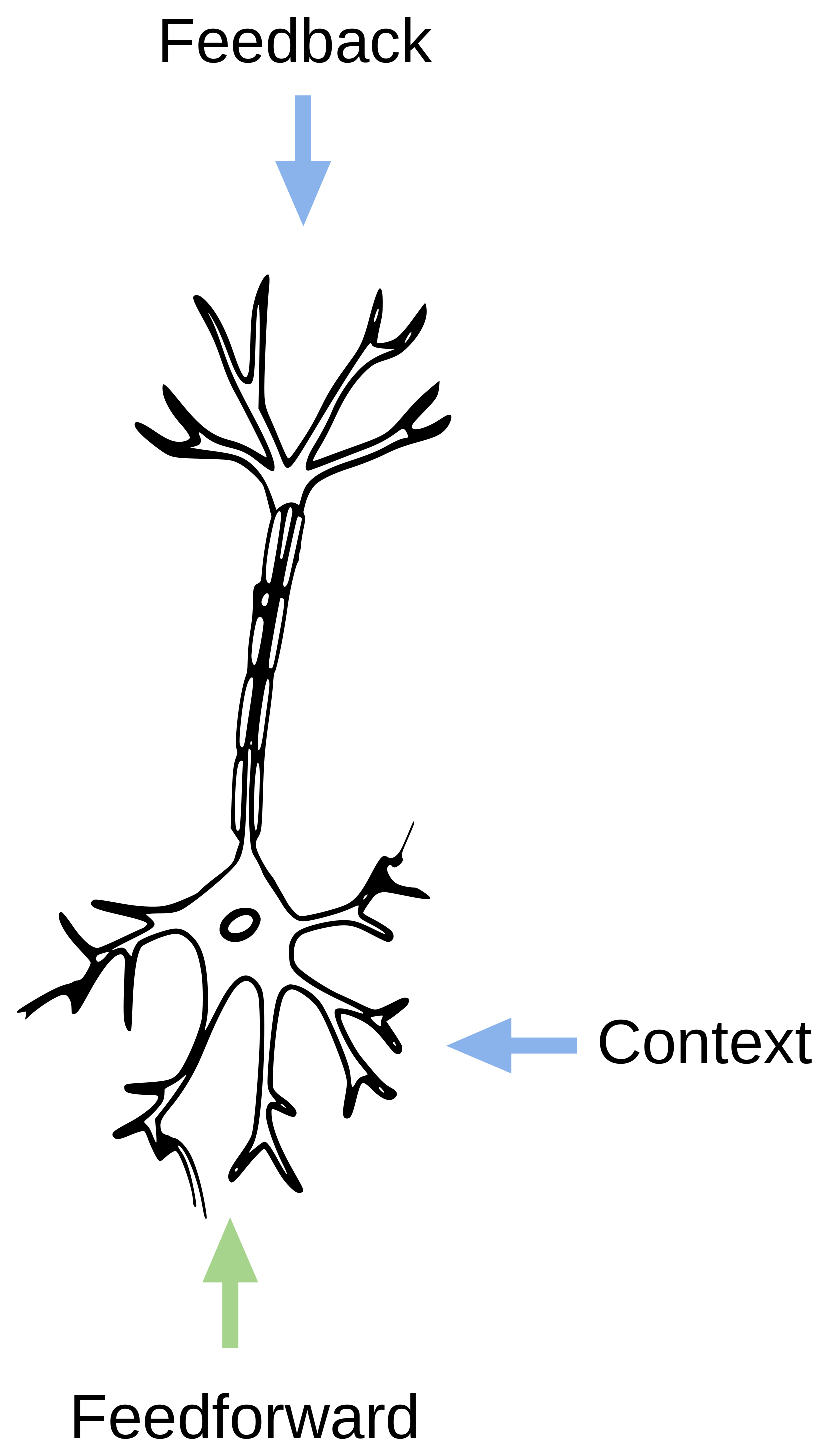
\includegraphics[width=\linewidth]{resources/related_works/neuron_biological}
        \caption{Biological neuron}
    \end{subfigure}
    \hfill
    \begin{subfigure}[b]{0.55\linewidth}
        \centering
        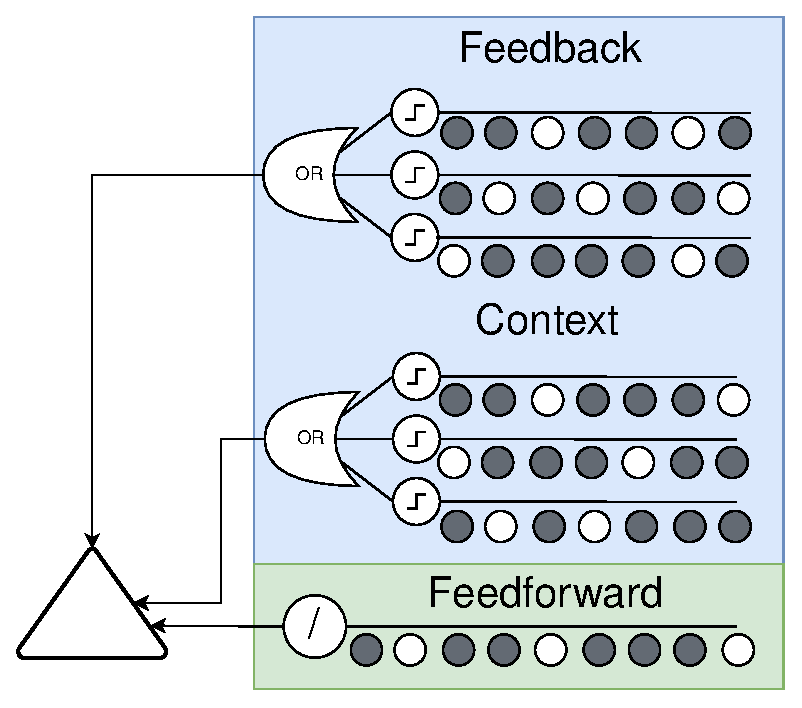
\includegraphics[width=\linewidth]{resources/related_works/neuron_htm}
        \caption[Comparison of neurons]{HTM neuron}
    \end{subfigure}
    \caption[Comparison of Neurons]{Comparison of neurons: Traditional Machine Learning (A), Biological Neuron (B), HTM Neuron (C). Source:~\cite{BAMI}}
    \label{fig:neuron_comparison}
\end{figure}
The HTM neuron has three inputs~\cite{htm_neurons}:
\begin{itemize}
    \item Feedforward, which is the input data
    \item Context, which is data from neighboring neurons and acts as a prediction mechanism for the next feedforward input
    \item Feedback, which is feedback from other neurons in the hierarchy and acts as a prediction mechanism for a sequence of feedforward inputs
\end{itemize}
How this type of neuron operates in HTM implementations will be covered in greater detail later in this section.
\subsection{Common Algorithm}
HTM theory states that there is a common algorithm for the intelligence. That the signals from hearing, vision, and touch are at the core processed by the same common algorithm. By extension, this means that HTM networks should be able to solve all kinds of logical tasks.
\subsection{Sparse Distributed Representation}
HTM theory introduces Sparse Distributed Representation (SDR) as a way of representing data in HTM and can be thought of as a bit-array. Each bit theoretically corresponds to a neuron in the neocortex and also represents some semantic information about the current data. This opens up for all kinds of mathematical operations, for instance it is possible to compare the semantic similarities between two SDRs by simply performing a binary AND operation, as seen in \autoref{fig:sdr_semantics}.
\begin{figure}[H]
    \centering
    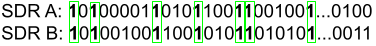
\includegraphics{resources/related_works/sdr-semantics.png}
    \caption[SDR Semantic Comparison]{Semantic similarities between the two SDRs A and B.}
    \label{fig:sdr_semantics}
\end{figure}
Observations of the brain has found that at any given point in time, a small percentage of neurons are activated and an SDR aims to keep this property by having a small percentage of bits be 1 at any given point. A common value is 2\% in order to mimic the sparsity of active neurons in the neocortex. Having this property means that the chance of two bit-patterns with different semantic meanings coinciding, for instance due to bit-flips caused by noise in the data, is astronomically low and is what makes HTM robust to noise. That being said, sparsity can be configured to be any value, as seen in \autoref{fig:sdr}.
\begin{figure}[H]
    \centering
    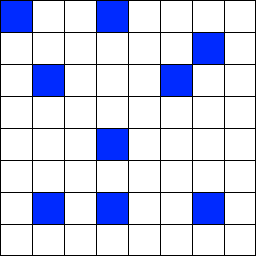
\includegraphics[width=0.25\textwidth]{resources/related_works/SDR.png}
    \caption[Example SDR]{Example representation of an SDR with a length of 64 and a sparsity of 14.1\%, visualized as a 2D grid.}
    \label{fig:sdr}
\end{figure}
\subsection{Encoders}
\label{sec:encoders}
To convert real-world data into an SDR, there is a need for an encoder in the pipeline. These encoders can be designed to take potentially any data and convert it into an SDR with an arbitrary sparsity. Given the fact that they may have an arbitrary sparsity, the output SDRs created by the encoder are sometimes referred to as just binary arrays.\par
Writing an encoder is no easy task as it is important to keep semantic similarities between values. This also means that the encoder is perhaps the most important part of an HTM pipeline to get right as it is the part that can limit the system the most. A biological example would be an eye that takes in visual information and converts it into an SDR so that it can be processed by the neocortex.
\par
There are principles that should be followed in order to create a good encoder:
\begin{itemize}
    \item Semantically similar data should result in SDRs with overlapping active bits
    \item The same input should always produce the same SDR
    \item The output must have the same dimensionality (total number of bits) for all inputs
    \item The output should have similar sparsity (similar amount of one-bits) for all inputs and have enough one-bits to handle noise and subsampling
\end{itemize}
As of now, there exists encoders for numbers, categories, geospatial locations, and dates. \autoref{fig:cyclical_encoder} shows a cyclical date encoding.
\begin{figure}[H]
    \centering
    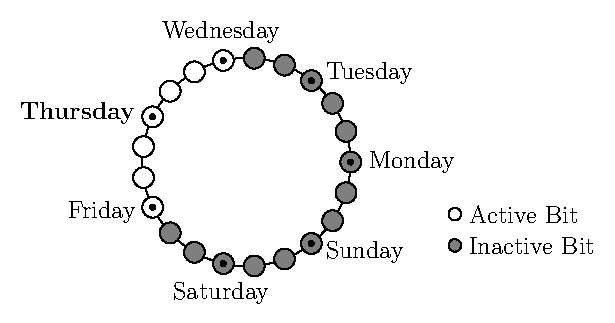
\includegraphics[width=0.9\linewidth]{resources/related_works/cyclical_encoder}
    \caption[Cyclical Date Encoding]{Visualization of a cyclical date encoding, which is currently encoding Thursday. Note that also Wednesday and Friday are included in the encoding of Thursday in order to emphasize that Wednesday and Friday are both equally distanced from Thursday.}
    \label{fig:cyclical_encoder}
\end{figure}
Some applications may require anomaly detection on multiple values at once, the correct approach then is to encode the values into SDRs one by one and then concatenate them into a single SDR before passing it to the HTM.
\subsubsection{Encoding Visual Data}
Several approaches for encoding visual data have been proposed. An example is a neuroscientifical approach which replicates how the eye works~\cite{eyeencoder}, another example is the approach by \textcite{ObjectDetectionSIFT} which uses scale-invariant feature transform (SIFT) to find points of interest in images and encode that information as an SDR. A simple threshold, as seen in \autoref{fig:binary_threshold_example}, can also be applied to extract information into an SDR-friendly format.
\begin{figure}[H]
    \centering
    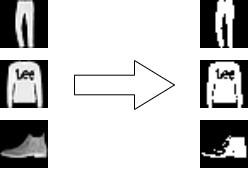
\includegraphics[width=0.5\linewidth]{resources/related_works/binary_threshold_example.png}
    \caption[Thresholding Example]{Example thresholding on the Fashion MNIST dataset~\cite{mnist_fashion}.}
    \label{fig:binary_threshold_example}
\end{figure}
\par
There are also deep learning approaches such as the one proposed by \textcite{CNN_HTM} which uses a Convolutional Neural Network (CNN) as part of the encoder. It creates an SDR by storing the top $n$-features in a feature map as ones and set the rest to zeros in order to achieve binary values suitable for the SDR.
\par
There are several reasons why these approaches might not perform well in videos. Keypoint detectors such as SIFT cause a lot of noise due to points shifting as lighting is changing. The distribution of the points within a frame is also constantly changing, which adds even more noise.
\par
The reason for why a direct binary threshold encoding might not perform well is due to the fact that it is neither position nor scale invariant and as such breaks the first principle of creating a good encoder. For instance, if it is desired that two pictures of the same object, but in different scales have more or less the same semantic meaning, then a direct binary encoding is not going to work. Direct binary threshold encoders also lead to loss of information, and is hard to perform for complex objects.
\par
An encoder which transforms convolutional feature maps into SDRs could be the answer, but the issue is converting the dense representation of the feature maps into SDRs. Directly encoding them into SDRs by treating each value in the feature map as a float and converting it into its own SDR quickly becomes intangible due to the processing and memory requirements. \autoref{fig:cnn_features} shows only a small subset of all the feature maps in a single layer, which highlights how intangible this approach is.
\begin{figure}[H]
    \centering
    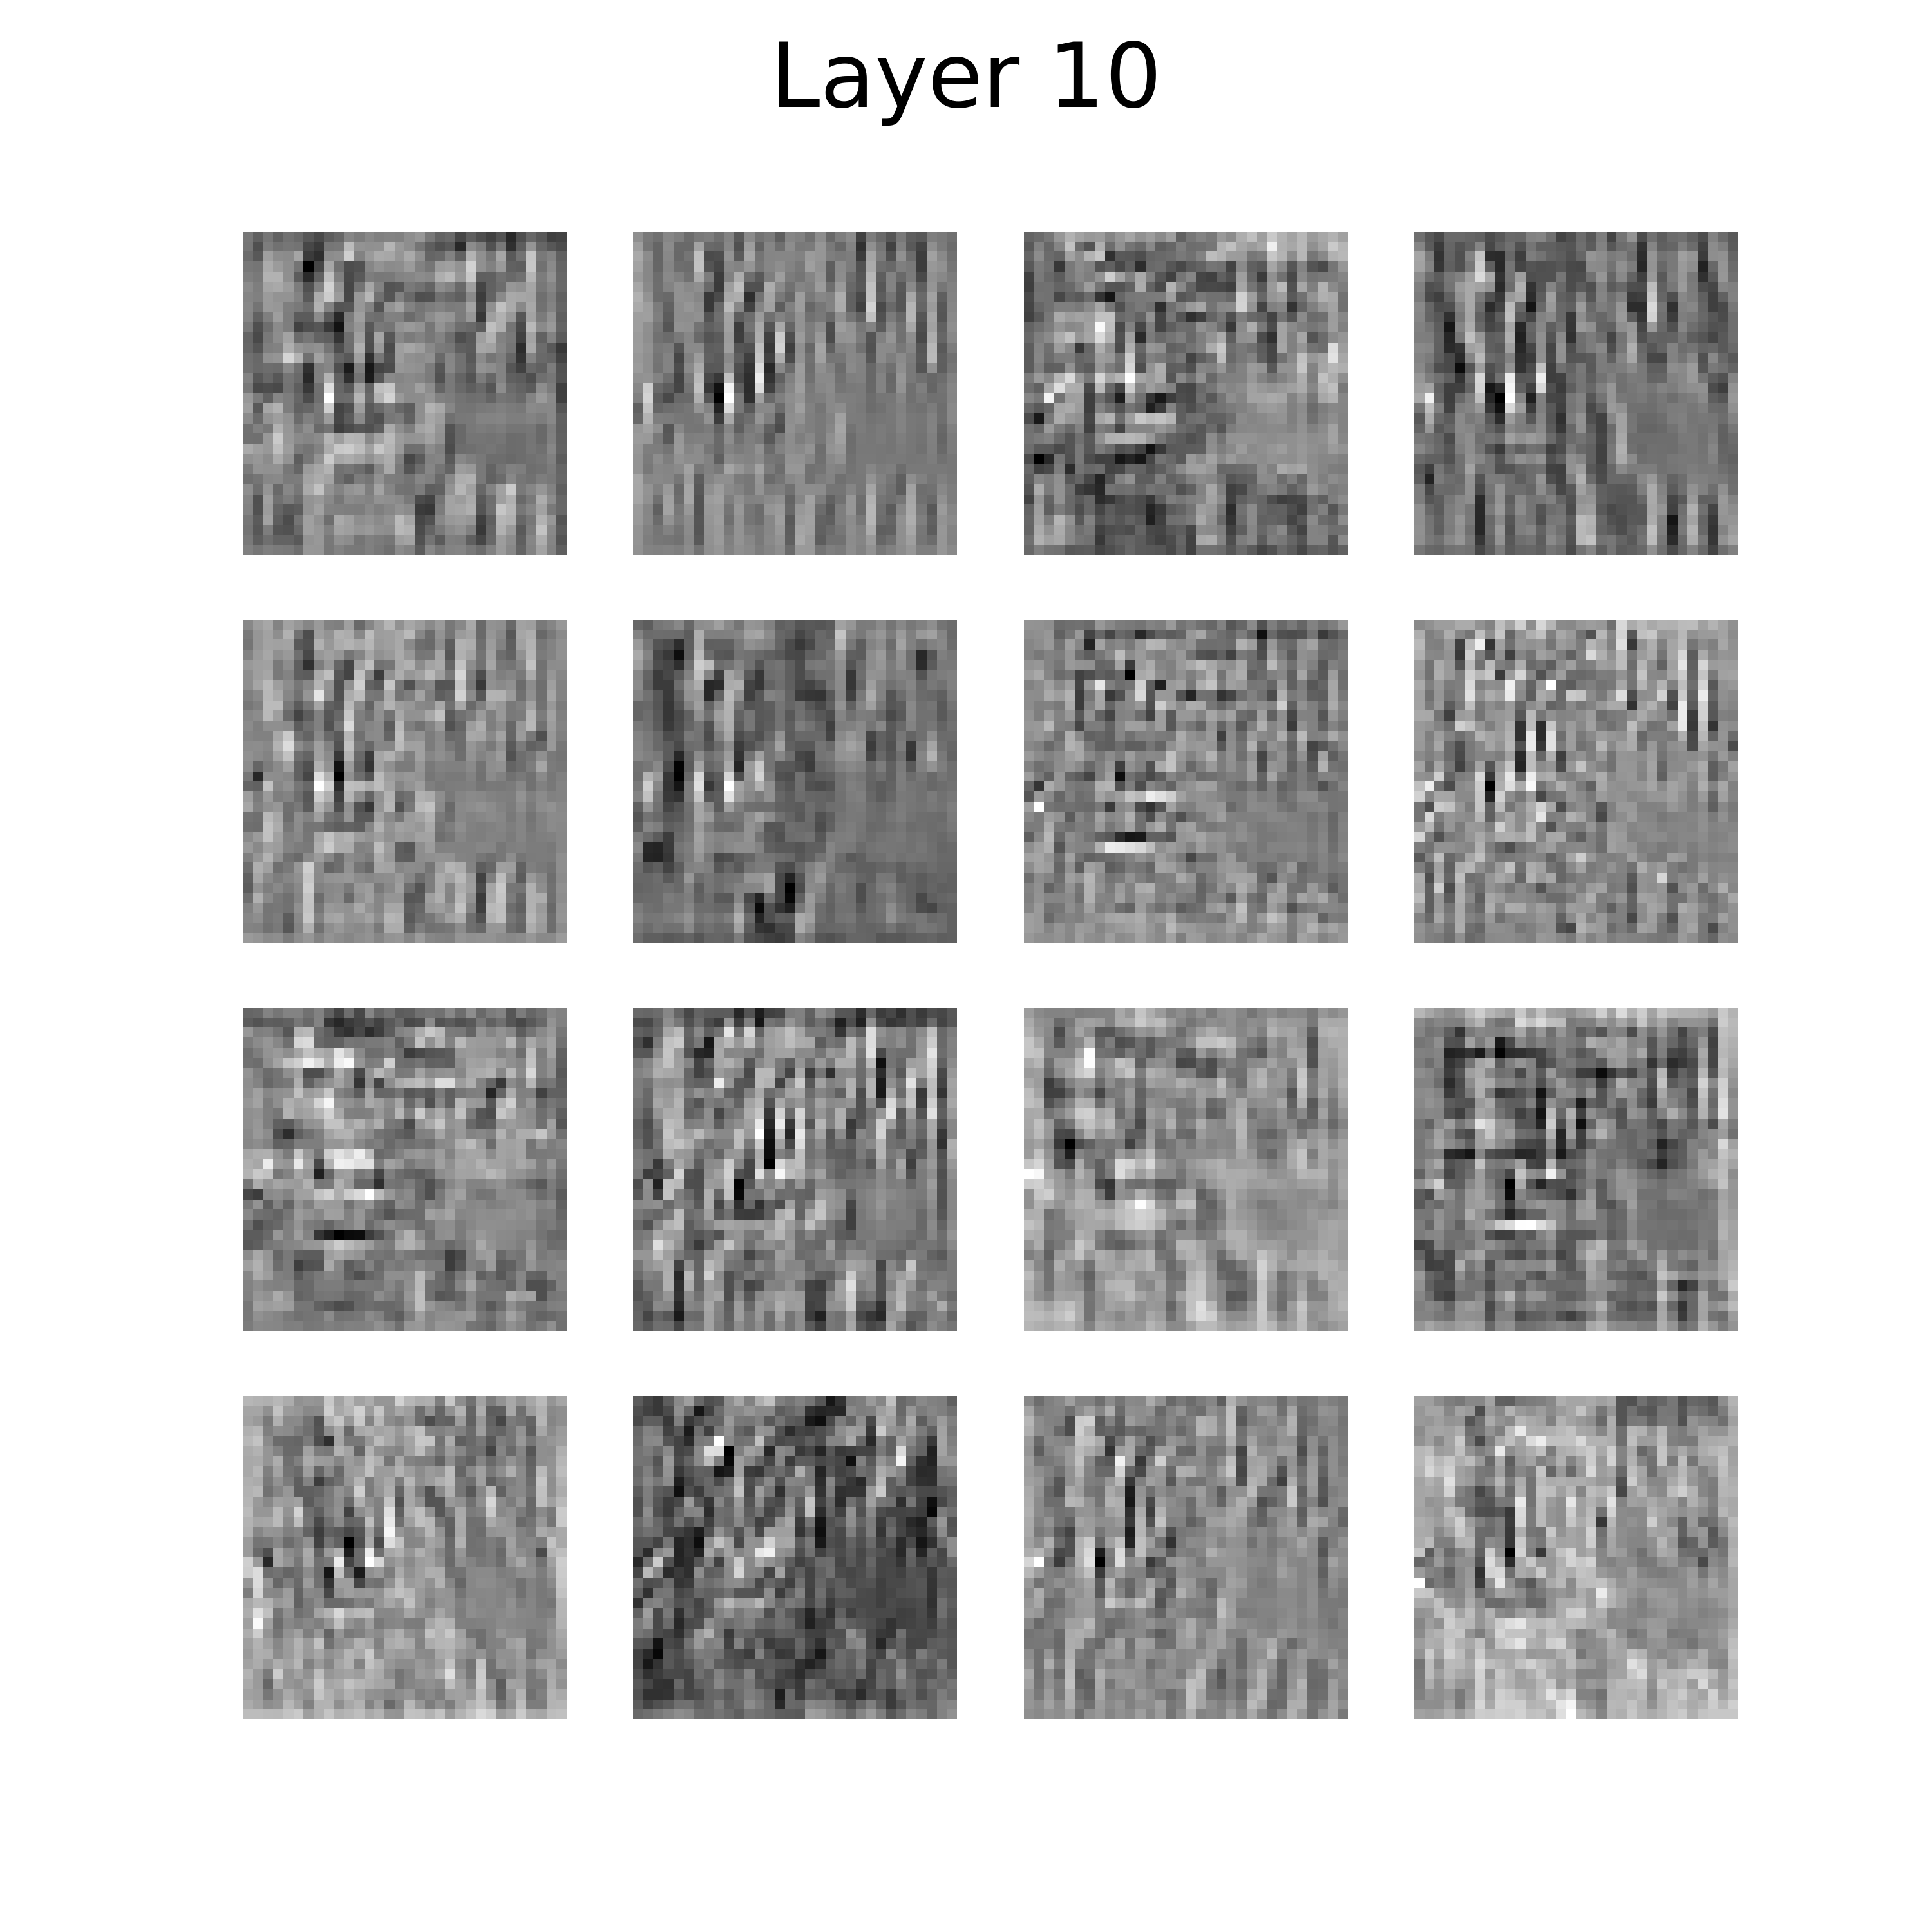
\includegraphics[width=0.5\linewidth]{resources/related_works/resnet18_layer_10.png}
    \caption[Feature Maps]{Select few feature maps in the 10th layer of ResNet18~\cite{resnet} trained on ImageNet~\cite{imagenet}.}
    \label{fig:cnn_features}
\end{figure}
\par
Additionally, minor variations in the feature map would cause major variations in the resulting SDR. Alternatively, one could follow \textcite{CNN_HTM} and binary threshold the top-$n$ features, but this leads to its own problems such as loss of information and that the information contained in the top-$n$ features is often undefined in models trained for complex tasks. It is also undefined what the top-$n$ features represent when there are no strong activations in the feature maps.
\par
Seeing as there is currently no encoder that can produce sensible SDRs from high dimensional data such as videos, a natural conclusion to make is that HTM should be applied differently, and that a new type of architecture using HTM should be explored for this purpose.
\subsection{Learning}
Similar to mammalian intelligence, HTM is designed to work on streaming data. It does not operate with batches like traditional machine learning, but rather with streaming data that may be changing over time. \par
The learning mechanism consists of two parts; the Spatial Pooler (SP) and the Temporal Memory (TM) algorithm. The latter is also commonly referred to as Sequence Memory. Together they make up multiple HTM neurons.\par
The spatial pooler takes SDRs produced by the encoder, and uses Hebbian like learning to extract semantically important information into output SDRs. These output SDRs usually have a fixed sparsity of about 2\% due to the fact that the spatial pooler aims to produce SDRs that have similar sparsity to what has been observed in the neocortex, but this can be configured at will and is dependent on the problem at hand.\par
The temporal memory algorithm, on the other hand, simulates the learning algorithm in the neocortex. It takes the SDRs formed by the spatial pooler and does two things:
\begin{itemize}
    \item Learns sequences of SDRs formed by the spatial pooler
    \item Forms a prediction, in the form of a predictive SDR,  given the context of previous SDRs
\end{itemize}
A typical HTM pipeline can be seen in \autoref{fig:htm_pipeline}.
\begin{figure}[H]
    \centering
    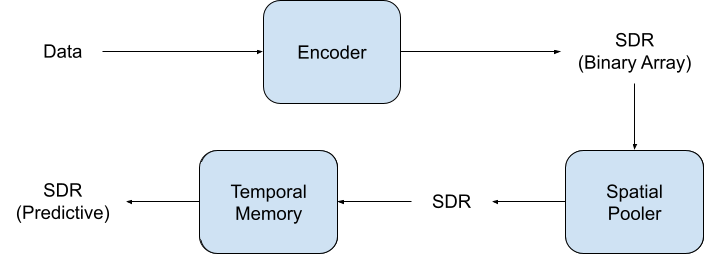
\includegraphics[width=\linewidth]{resources/related_works/htm_pipeline.png}
    \caption[The HTM Pipeline]{A typical HTM pipeline. A common next-step could be to use a classifier to convert the predictive SDR into a classification. }
    \label{fig:htm_pipeline}
\end{figure}

This learning mechanism gives HTM systems the property of on-line learning, meaning they learn as they go. There is no batch training because each input into the HTM system will update the system. The system effectively builds a predictive model of the data and learns by trying to minimize the error between the true values and the predicted values. This means that the system will continuously adapt to a changing environment.
\begin{figure}[H]
    \centering
    \begin{subfigure}[b]{0.35\linewidth}
        \centering
        \hspace*{1cm}
        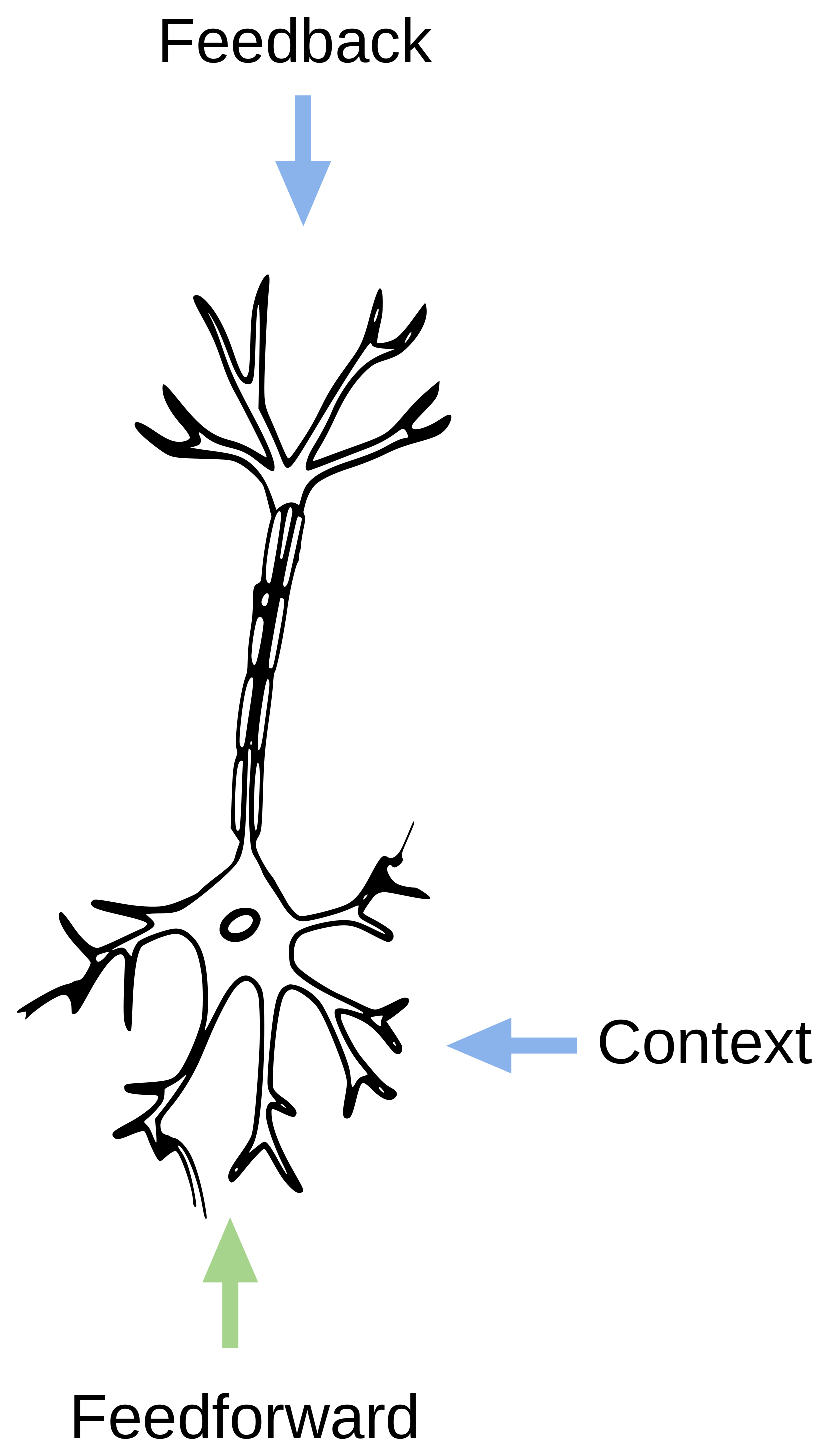
\includegraphics[width=\linewidth]{resources/related_works/neuron_biological}
        \caption{Biological neuron}
    \end{subfigure}
    \hfill
    \begin{subfigure}[b]{0.55\linewidth}
        \centering
        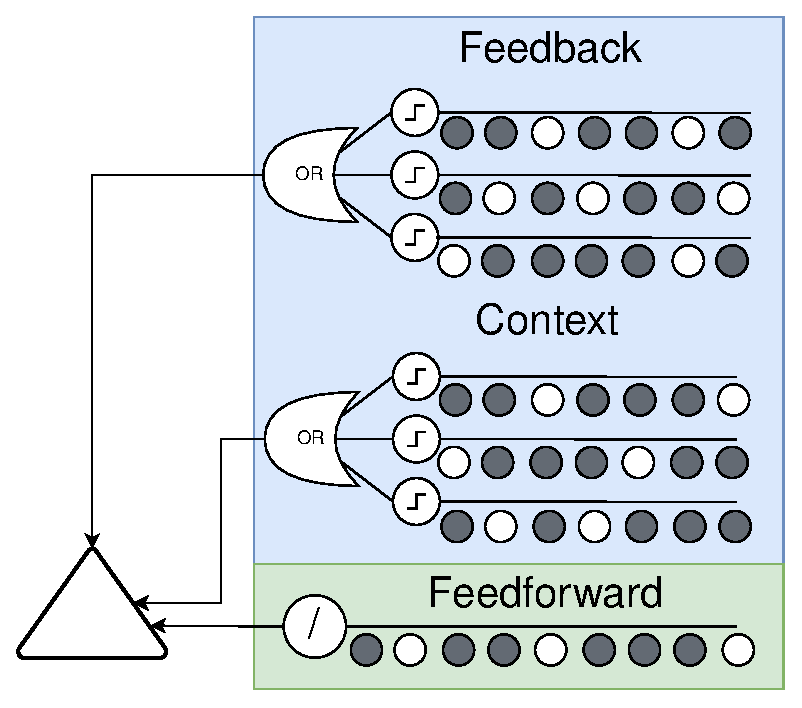
\includegraphics[width=\linewidth]{resources/related_works/neuron_htm}
        \caption{HTM neuron}
    \end{subfigure}
    \caption[SP and TM Responsibilities]{Biological neuron and HTM neuron, the colors show which part the SP and the TM covers.}
    \label{fig:sp_tm_responsibility}
\end{figure}
\autoref{fig:sp_tm_responsibility} shows that a spatial pooler combined with a temporal memory forms the HTM neuron, where the color green indicates the responsibility of the Spatial Pooler and blue indicates the responsibility of the Temporal Memory.
\subsubsection{Spatial Pooler}
\label{sec:spatial_pooler}
The spatial pooler consists of columns (mini-columns), where each column has a receptive field covering the input. In technical implementations of spatial poolers, the columns exist in name only and could be thought of as nodes instead. A column can cover parts of the input or the entire input, the range being referred to as the \textbf{potential radius}. During initialization, each column creates random connections to a percentage of the bits in the input space within its receptive field, this gives each column a unique \textbf{potential pool} when there are overlaps of receptive fields caused by a large potential radius. This is visualized in \autoref{fig:sp_vis_alt}.\par
\begin{figure}[H]
    \centering
    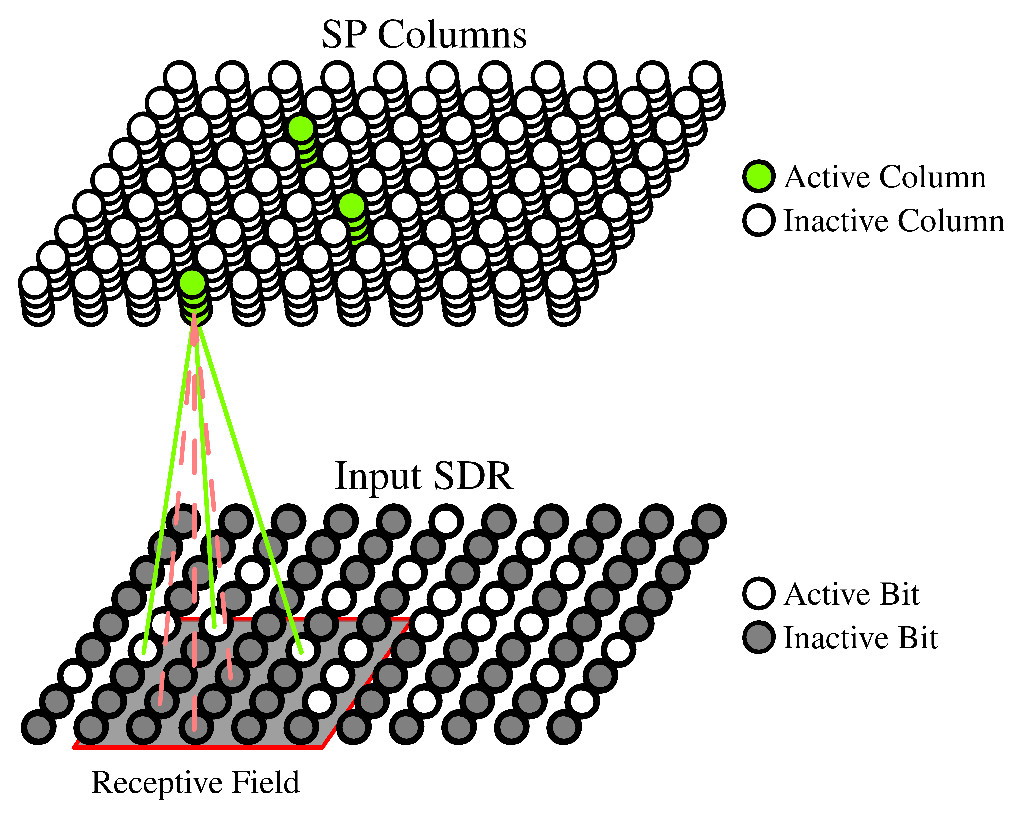
\includegraphics[width=\linewidth]{resources/related_works/sp_vis_alt}
    \caption[Spatial Pooler Visualization]{Visualization of the \gls*{sp} and the potential pool of one of its columns.}
    \label{fig:sp_vis_alt}
\end{figure}
Each connection is described using a \textbf{permanence}-value which can be considered the "strength" of the connection, and it ranges between 0 and 1. During learning, the permanence value of the connections is increased or decreased depending on whether the corresponding bit in the input is active or inactive. When the permanence-value crosses above a \textbf{stimulus threshold}, the connection will be considered "active".

The amount of active connections for a given column is referred to as \textbf{overlap score}. If a column has a high enough overlap score which crosses the \textbf{overlap score threshold}, then the column will itself become active. The reason behind locking activation behind a minimum overlap score is to reduce the influence of noise in the input. Finally, out of all the active columns, only the top $n$ columns with the most overlap score will be selected to be included in the \gls*{sp} output. The value $n$ is chosen so that the \gls*{sp} output has a specific \textbf{sparsity}. Only the selected columns are allowed to learn (increase/decrease permanence). \autoref{fig:sp_vis} visualizes the mechanism that determines the output in the SP.
\par
\begin{figure}[H]
    \centering
    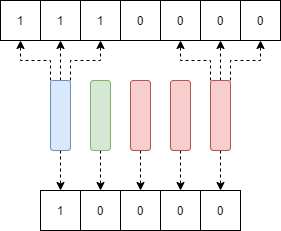
\includegraphics[width=0.6\textwidth]{resources/related_works/sp_vis.png}
    \caption[Spatial Pooler Workings]{ This figure illustrates how a spatial pooler works. All connections are above the stimulus threshold. The receptive field is 3 bits wide for each column. Overlap score threshold is $1$, and $n=1$. Red means inactive, green means active, and blue means active and selected.}
    \label{fig:sp_vis}
\end{figure}
Because only the active columns are allowed to learn, only a select few columns who got lucky during the random initialization will dominate the spatial pooler output and have a very high \textbf{active duty cycle}. Active duty cycle measures how often a column is active and ranges from 0 (never) to 1 (always). \par
To counter dominating columns, the spatial pooler uses \textbf{boosting}.
The concept behind boosting is to "boost" the overlap score of underperforming columns and lower the overlap score of over performing columns. The result is that more columns learn and contribute to the output, which means that the spatial pooler can then process the input data with a finer granularity. This is also a form of regularization. One has to be careful with boosting, since it can cause instability in the spatial pooler output.
\par
It is also possible to have \textbf{topology} in the output by selecting the columns to be included in the output by their local neighborhood, instead of comparing their overlap score globally.
\par
All the aforementioned concepts are configurable in technical implementations.

\subsubsection{Temporal Memory}
\label{sec:temporal_memory}
The temporal memory consists of the columns that a spatial pooler outputs, but treats them as actual columns instead of "nodes". These columns consist of cells and can contain an arbitrary \textbf{number of cells} which defines the capacity of contexts that the temporal memory can express. Each cell in a column can connect to other cells in other columns using segments (more specifically, distal dendrite segments), where each segment consists of synapses connecting to other cells.
\par
Essentially, it takes the "node" based representation of the \gls*{sp} output, and turns it into a new representation which includes state, or context, from previous time steps. It achieves this by only activating a subset of cells per column, typically only one per column. This allows the temporal memory to represent a pattern in multiple contexts. If every column has 32 cells and the \gls*{sp} output has 100 active columns and only one cell per column is active, then the \gls*{tm} has $32^{100}$ ways of representing the same input. The same input will make the same columns active, but in different contexts different cells in those columns will be active. This is visualized in \autoref{fig:tm_vis_alt2}.
\begin{figure}[H]
    \centering
    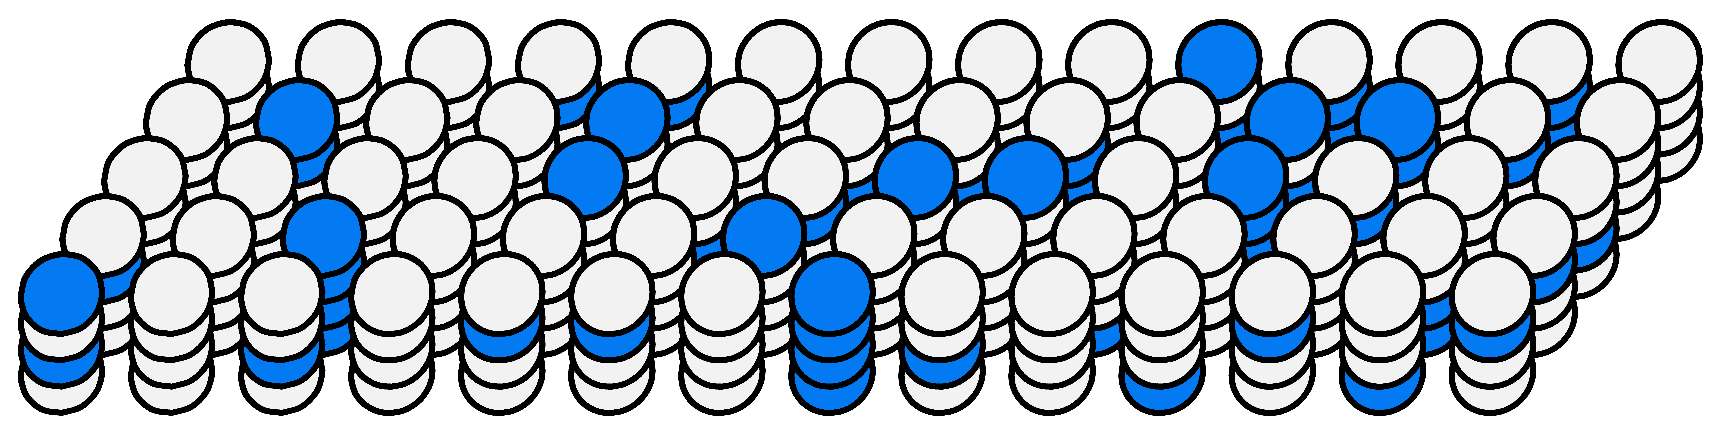
\includegraphics[width=\linewidth]{resources/related_works/tm_vis_alt2}
    \caption[Temporal Memory Visualization]{Visualization of the TM, with number of cells equal 4. Some columns are bursting.}
    \label{fig:tm_vis_alt2}
\end{figure}
\par
The temporal memory algorithm consists of two phases. The first phase is to evaluate the \gls*{sp} output against predictions and choose a set of active cells. It does so by looking at the active columns and the cells they contain. If an active column contains predictive cells, then those cells are marked as active. If an active column has no predictive cells, usually caused by observing a new pattern for the first time, then the column "bursts" by activating all the cells that the column contains (see \autoref{fig:tm_vis1}). Otherwise, a cell is inactive.
\par
\begin{figure}[H]
    \centering
    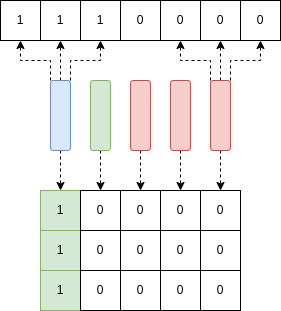
\includegraphics[width=0.6\textwidth]{resources/related_works/tm_vis1.png}
    \caption[Temporal Memory Workings]{Expanded \gls*{sp} example with \gls*{tm} component where the number of cells is set to 3. The leftmost column is bursting (all 3 cells activated in green) due to the active \gls*{sp} output and due to containing no predictive cells.}
    \label{fig:tm_vis1}
\end{figure}
At this point, the active cells represent the current input in the context of previous input. For each active column we look at the segments connected to the active cell(s). If the column is bursting we look at the segments that contain any active synapses, if there is no such segment we grow one on the cell with the fewest segments. On each of the segments that we are looking at, we \textbf{increase the permanence} on every active synapse, \textbf{decrease the permanence} on every inactive synapse, and grow new synapses to cells that were previously active. The algorithm also punishes segments that caused cells to enter predictive state, but which did not end up being active.
\par
Since the \gls*{tm} can only grow synapses to cells that were active in the previous timestep, the \gls*{tm} struggles to express sequences of patterns over multiple timesteps, as has been discussed on HTM forums~\cite{tm_sequence_problem}. The solution has been to also encode some temporal information, such as the time of day~\cite{AHMAD2017134,tm_sequence_problem}, so that it can use timestamps as anchor points for its contexts.
\par
The second phase is to form a prediction by putting cells into a predictive state. For every segment on every cell, the number of synapses connected to active cells are counted. If the number exceeds an \textbf{activation threshold}, then the segment is marked as active and all the cells connected to the segment enter the predictive state. To summarize, a cell has three possible states:
\begin{itemize}
    \item Active, if the column is bursting or the cell was in a predictive state in the previous time step and the column it belongs to is active.
    \item Predictive, if a connected segment is active, which is in turn determined by the amount of active synapses.
    \item Inactive, if none of the other states apply.
\end{itemize}
\autoref{fig:tm_vis_alt} visualizes cells with different states in the TM.
\begin{figure}[H]
    \centering
    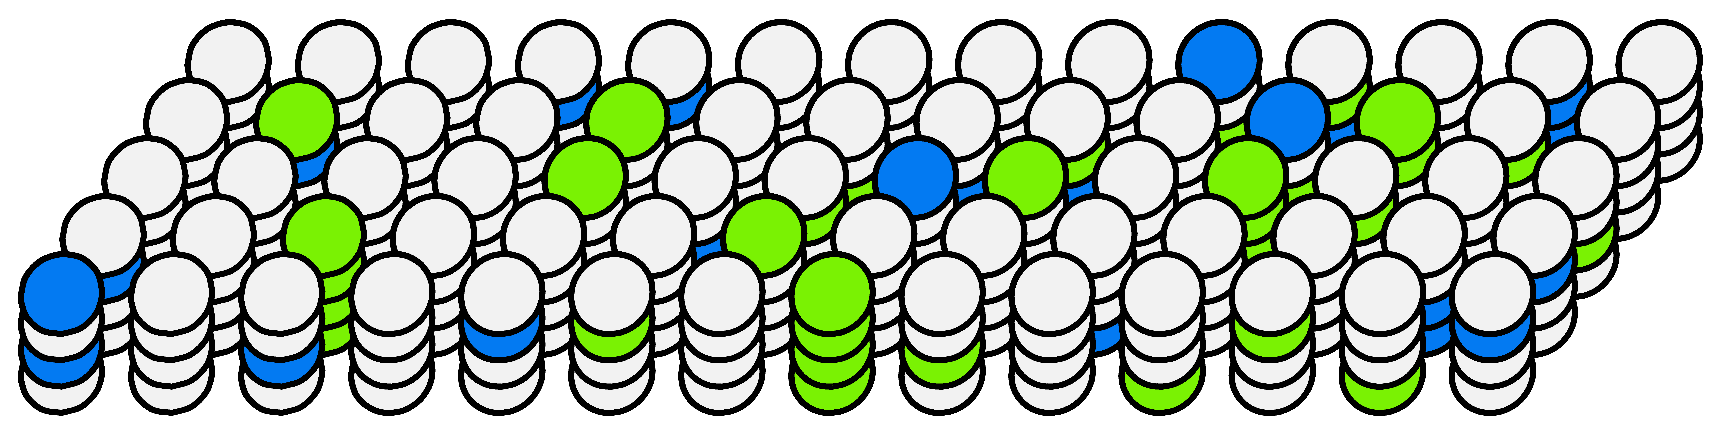
\includegraphics[width=\linewidth]{resources/related_works/tm_vis_alt}
    \caption[Visualization of Cell States]{Visualization of the \gls*{tm} and the three states. Active in green, predictive in blue, and inactive in white.}
    \label{fig:tm_vis_alt}
\end{figure}

One can configure how much the system can learn by setting the number of cells and the values by which permanence should be increased or decreased. If it is desired that the \gls*{tm} does not "forget" at all, then the permanence value by which synapses are decremented can be set to 0. If it is desired that the \gls*{tm} can only express patterns in the current context and the context of the previous time step, then the number of cells can be set to 2.
\par
Finally, the \gls*{tm} compares the predictions $P_{t-1}$ it made in the previous time step with the actual pattern $A_t$ in the current time step and calculates an anomaly score:
\begin{align*}
    anomalyScore=\frac{|A_t-(P_{t-1}\cap A_t)|}{|A_t|}
\end{align*}
Which is a normalized value from 0 to 1. If the anomaly score is 1, then it means that none of the predicted columns matched the current active columns of the spatial pooler. If it is 0, then it means that all predicted columns matched the current active columns of the SP.\par
It is also possible to estimate the number of predictions being made by the \gls*{tm} at any time~\cite{htm_predictions_count}. This is done by counting the number of predictive cells, and dividing them by the number of active bits required to express a pattern. As an example, if sparsity is set so that patterns have 60 active bits and the number of predictive cells is 120, then the estimated number of predictions is given as
\begin{align*}
    numPredictions=\frac{predictiveCells}{activeBits}=\frac{120}{60}=2
\end{align*}
This is only an estimation, in reality the two patterns may have overlapping bits in their representations, and the number of active bits for each representation may have minor deviations.
\subsection{Use Cases}
The general use case for HTM is to perform anomaly detection. More specifically, Numenta has made example applications showcasing how HTM can be used in practice~\cite{numenta_example_apps}:
\begin{itemize}
    \item \textbf{Rogue Behavior Detection} which models normal behavior and detects anomalies, such as unusual use of files in a network~\cite{htm_rogue}.
    \item \textbf{Geospatial Tracking} which detects anomalies in the movement of people, objects, or material, using speed and location data~\cite{htm_geospatial}.
    \item \textbf{Financial Monitoring} which detects anomalies in publicly traded companies by continuously modelling stock price, stock volume, and Twitter volume~\cite{htm_finance}.
\end{itemize}
There are other examples on the use of HTM for real world applications. One of them is the work done by \textcite{htm_medicine}, which showcases how HTM can be used to model medical streams in real time. Another example is the work done by \textcite{htm_electrical_load}, which shows how HTM can be used for forecasting electrical loads in power grids.
\par
There are also applications that are actively used in production, such as the model offered by \href{www.cortical.io}{cortical.io} which builds upon HTM in order to perform language analysis. This is made this possible by introducing Semantic Folding and Semantic Fingerprinting~\cite{semantic_folding}.
\subsection{The Thousand Brains Theory}
One of the newest advancements in HTM Theory is the introduction of the Thousand Brains Theory. \textcite{thousandbrains} introduces the Thousand brains theory as a way of redefining hierarchy in the brain based on recent neuroscientifical discoveries. Instead of our classical understanding of hierarchy in deep learning where each layer takes simple features and outputs complex features, we now have that every layer of the hierarchy sees the input at once but at different scales and resolutions. The different nodes in the hierarchy are now also connected and thus enable the network to use all available views of the object in order to create an understanding of that object. \par
To summarize, the object is learned by the brain using multiple models that may rely on different inputs, the models then vote to reach a consensus on what they are sensing. This is coincidentally similar to ensemble learning such as \textcite{divergentNets}. Each model can be thought of as a mini-brain, hence the name "The Thousand Brains Theory".
\begin{figure}[H]
    \centering
    \begin{subfigure}[t]{0.55\textwidth}
        \centering
        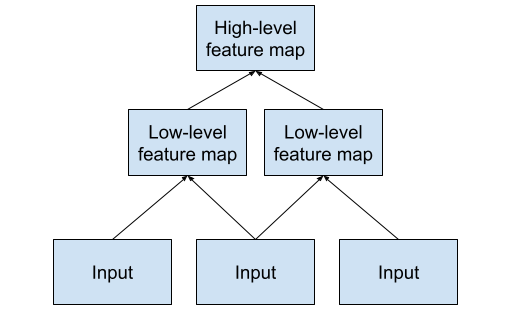
\includegraphics[width=1\linewidth]{resources/related_works/hierarchy.png}
        \caption{Classical Hierarchy}
        \label{fig:my_label}
    \end{subfigure}
    \hfill
    \begin{subfigure}[t]{0.3\textwidth}
        \centering
        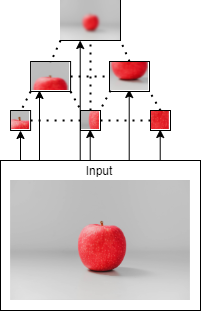
\includegraphics[width=1\linewidth]{resources/related_works/thousand_brains.png}
        \caption{Hierarchy as in the Thousand Brains Theory}
        \label{}
    \end{subfigure}
    \caption[Thousand Brains Visualization]{Comparison of classical hierarchy and the hierarchy introduced by the Thousand Brains Theory.}
\end{figure}
This new type of hierarchy is also quite similar to some state-of-the-art image recognition deep learning architectures such as InceptionNet~\cite{inceptionnet} (see \autoref{fig:inception_module}) and Feature Pyramid Networks~\cite{fpn}, in the sense that they apply different sized convolutional filters, where each filter can be thought of as its own separate model, on the data and do predictions based on all of them at once. This also ensures scale invariance of objects fed in to the architecture.
\begin{figure}[H]
    \centering
    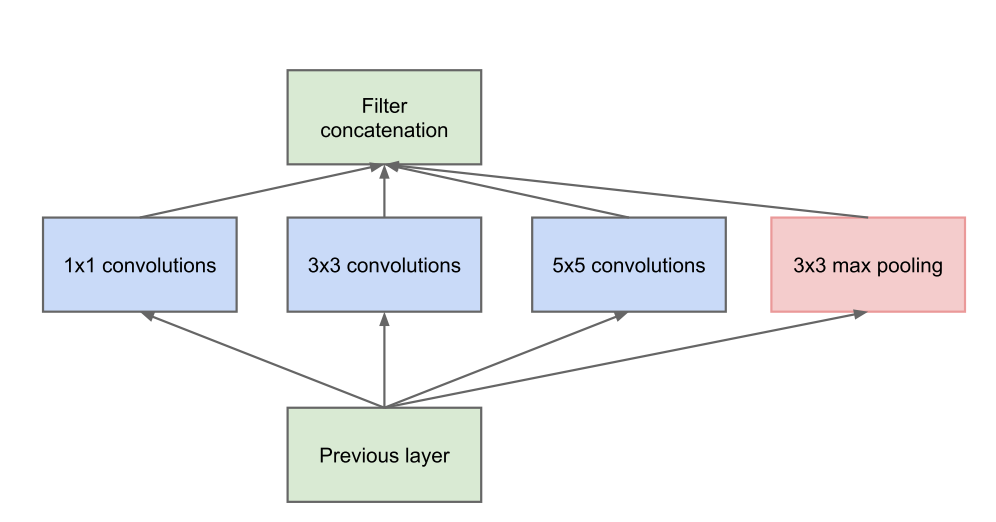
\includegraphics[width=\linewidth]{resources/models/inception_module.png}
    \caption[Filter Concatenation]{How the Inception~\cite{inceptionnet} architecture uses multiple filters at once.}
    \label{fig:inception_module}
\end{figure}

While the Thousand Brains Theory is not yet technically implemented in any way in a standard HTM model, it does show that recent developments within deep learning for image analysis have similarities with HTM theory.

\subsection{HTM Performance in Anomaly Detection}
\label{sec:htm_perf}
Knowing that deep learning approaches have a high degree of accuracy but suffer from problems related to generalizability, adaptability, and noise it stands to reason that HTM is a viable alternative for anomaly detection.\par
\textcite{AHMAD2017134} explores the use of HTM for anomaly detection on low dimensional data such as temperature data from an industrial machine. The authors also discuss benchmarks for anomaly detection and compare different methods. The results show that HTM is very capable of performing anomaly detection, especially in a changing environment. HTM is able to outperform other anomaly detection methods and has the advantage of not requiring any per-problem parameter tuning.
\par
For high-dimensional anomaly detection; \textcite{MotionAnomalyDetection} used a HTM system to find anomalous frames in videos of motions (\autoref{fig:motion_frame}). The anomalies were artificially created by swapping certain frames between different motion videos in the dataset. The results show that the HTM system was able to correctly detect some anomalies, but not an impressive amount.
\begin{figure}[H]
    \centering
    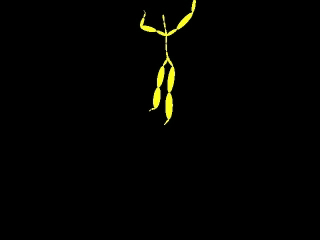
\includegraphics[width=0.5\linewidth]{resources/related_works/motion_frame.png}
    \caption[Example Motion Frame]{Example motion frame~\cite{MotionAnomalyDetection}.}
    \label{fig:motion_frame}
\end{figure}
One thing to note is that direct binary representations of the video frames were used as SDRs, therefore no proper encoding was performed which might have led to the poor results. This hints at the fact that HTM by itself is not capable of handling high dimensional data, and is instead reliant on an encoder to lower the dimensionality by extracting important spatial features.
\section{Ethical Considerations}
This thesis introduces an architecture for performing surveillance on potentially a massive scale, and could even be tied to some sort of social credit system. This raises ethical questions regarding mass surveillance that highlight how the work done in this thesis can be misused. Therefore, even if the work done in this thesis is nowhere near perfect and far from ready to be used in production, one should still keep the ethical aspects in mind when pursuing this type of research.
\par
It should also be reiterated that HTM is the result of research from a private company, which is why one should be extra critical of their work. Another aspect is that unlike deep learning, which is democratized, HTM is still very centralized. This means that Numenta has a lot of influence within the development of HTM, which could be misused for the purpose of promoting the goals of the company.
\section{Summary}
Deep learning can be traced back to the Perceptron which was a machine learning model capable of solving linearly separable problems. Over time, people theorized that stacking Perceptrons would give it the ability to solve more complex problems. This was not possible before back propagation was introduced. After that, deep learning evolved and new architectures were invented. One of the main contribution is the introduction of the CNN, which allowed deep learning approaches to achieve state-of-the-art results for complex problems such as image classification. The ability to train deep learning on the GPU and the introduction of frameworks caused deep learning to explode in popularity. One of the latest advancements is the introduction of generative models, which can be used for various purposes including generating realistic data. Deep learning has several issues, such as lack of explainability, the need for a lot of data, and poor out-of-distribution performance.
\par
Anomaly detection is often defined as detecting data points that deviate from the general distribution. Unlike most other problems in deep learning, anomaly detection deals with unpredictable and rare events which makes it hard to apply traditional deep learning for anomaly detection. Popular approaches therefore often employ generative models, that calculate an anomaly measure using generated or reconstructed data. A subset of anomaly detection is smart surveillance, which is the use of video analysis specifically in surveillance. Recent developments show that generative models have a high degree of accuracy and are consistently improving.
\par
HTM theory introduces a machine learning algorithm which works on the same principles as the brain and therefore solves some of the issues that deep learning has. HTM is considered noise resistant and can perform online learning, meaning that it learns as it observes more data. HTM replicates the structure of the neocortex which is made up of cortical regions, which in turn are made of up of mini-columns and then neurons. HTM neurons are more complex than neurons in deep learning, and perform learning with Hebbian-like learning. The data in an HTM is represented using an SDR, which is a sparse bit array. An encoder converts real world values into SDRs. One of the difficulties with HTM is making it work on visual data, where creating a good encoder for visual data is still being researched. The learning mechanism consists of two parts, the spatial pooler and the temporal memory. The spatial pooler learns to extract semantically important information into output SDRs. The temporal memory learns sequences of patterns of SDRs and forms a prediction in the form of a predictive SDR. Research has shown that HTM is very capable of performing anomaly detection on low-dimensional data and is able to outperforms other anomaly detection methods. However, related works show that HTM struggles with higher dimensional data.